\begin{history}

    \subsubsection*{1875-1900}

    Die Wiegenjahre brachten der Musikgesellschaft Hildisrieden
    abwechslungsreiche Begebenheiten.

    Die Hauptbetätigung blieb weiterhin das Konzertieren in Form von Ständchen
    und Ausmärschen, in und ausserhalb der Gemeinde. So treffen wir die
    Musikgesellschaft 1882 im Emmenbaum anlässlich einer Theateraufführung und
    1887 beritten am Auffahrtsumritt in Sempach. Die Entschädigung, welche die
    Musikgesellschaft von der Kirchenverwaltung Sempach erhielt, betrug immerhin
    45 Franken. Ein Gesuch, den Auffahrtsumritt abwechslungsweise mit der
    Musikgesellschaft Sempach alle drei Jahre bestreiten zu dürfen, wurde von
    der Kirchenverwaltung abgelehnt.

    Was unseren Musikanten in den 1890er Jahren vorgeworfen werden konnte, war
    der Mangel an Ordnung  und Disziplin. Wohl hatte man 1884 neue Statuten
    aufgestellt und neue Strafbestimmungen festgesetzt; diese sind aber nicht
    von allen befolgt worden. Diese unruhigen Vereinsjahre, fünf an der Zahl,
    hatten zur Folge, dass man mit dem Gedanken spielte, die Musikgesellschaft
    aufzulösen oder sich den gegebenen Statuten zu fügen.

    Man fand sich hin und wieder zusammen und kam ebenso schnell wieder
    auseinander, bis schliesslich die Vernunft siegte. Ein weiterer Grund, der
    den Zusammenhang des Vereins trübte, war der kleine finanzielle Beitrag der
    Gemeinde. Jährlich 20 Franken waren wirklich kein grosses Honorar, wenn man
    bedenkt, dass jeder Musikant sein Instrument selbst zu beschaffen und die
    Musikgesellschaft an sämtlichen Prozessionen teilzunehmen hatte.

    Im Jahre 1899 wurde das Restaurant Kreuz eröffnet und der Saal im Löwen
    eingeweiht. Die Einladung zu diesen Festen fügte das schwache Gebilde wieder
    zusammen.

    Die Statuten von 1874 und 1884 erneuert, haben 10 Mitglieder unterzeichnet.
    Es sind: Silvester Schnieper, Josef Wolf, Leonz Geisshüsler, Silvester
    Disler, Josef Disler, Peter Troxler, Peter Muff, Rudolf Bühlmann, Josef Wolf
    und Niklaus Süess.

    Weitere Einnahmen wurden mit dem \enquote{Umblasen}  während der
    Weihnachtszeit in der Gemeinde erzielt. Vor den Häusern wurde jeweils
    musiziert, wofür die Musik-freundlichen Bewohner eine Geldgabe spendeten. Im
    Jahre 1886 brachte der Verein auf diese Weise Fr. 259.60 zusammen. Bei
    kaltem Wetter war das Musizieren kein Vergnügen, denn öfters froren die
    Ventile ein und mussten durch Einhauchen wieder beweglich gemacht werden.
    Gerne wurde dann die Einladung angenommen, ins Haus zu kommen.

    In der warmen Stube liess es sich bequemer musizieren, besonders da, wo auch
    \enquote{Mittel} gegen trockene Kehlen bereitstanden. Allzu lange aber
    durfte die Gastfreundschaft nicht beansprucht werden, warteten doch noch
    viele Einwohner auf den Besuch der Musikanten. War aber dann das gesteckte
    Tagesziel erreicht, wurde es mit dem Aufbruch nicht so genau genommen, gar
    wenn es oft etwas Feines zum Beissen gab.

    Leider ist nun auch dieser alte Brauch verschwunden. Dass es hin und wieder
    gemütlich wurde, berichtet die Chronik. Als beim Ausflug auf den Napf ein
    Leiterwagen mit Blumen und Girlanden geschmückt dem Sempachersee entlang
    rasselte, löste sich vom Wagen ein Rad, sodass ein Musikant nach dem andern
    vom Wagen kippte. Dabei gab es einige defekte Instrumente. Diese konnten in
    Willisau beim Instrumentenmacher Badmann wieder hergestellt werden. Die
    Fahrt führte ins Luthernbad und von da an zu Fuss auf den Napf. Dem
    Bassisten Troxler war das Bergsteigen nicht besonders angenehm, denn er soll
    sich damals geäussert haben: \enquote{Dass mer au uf ne so ne
        Morgelandssiech cha go!}

    \subsubsection*{Erste Fahnenweihe 1881}

    Nach dem schönen Erfolg am Musikfest in Münster, beschlossen Töchter des
    Dorfes unter der Initiative von Nanette Jutz, vom Löwen, und der Katharina
    Wolf, vom Sigristenhaus, eine Fahne anzuschaffen. Mit einem Symbol wollten
    sie den Musikanten eine Freude machen. Das nötige Geld wurde
    zusammengebettelt. Der Stoff war aus doppelter weisser Seide. Die
    Aufschriften und Zeichnungen wurden vom Malermeister Dolder in Münster
    ausgeführt. So war auf der Vorderseite geschrieben:
    \enquote{Musikgesellschaft Hildisrieden 1881} und in der Mitte war das
    Kantonswappen von einem Lorbeerkranz umgeben. Auf der Rückseite war zu
    lesen: \enquote{Wo Musiktöne lieblich klingen, hebt sich das Herz auf
        Adlerschwingen}. Dieser Spruch war mit einem Eichenkranz umgeben. Eine Harfe
    mit Notenbuch umrahmte diesen Spruch. Die Übergabe fand in ganz einfachem
    Rahmen auf dem Dorfplatz statt, gestaltete sich aber zu einem urgemütlichen
    Volksfest.

\end{history}

\begin{figure}[ht]
    \centering
    \subfloat[alte Kirche mit Pfarrhaus]{%
        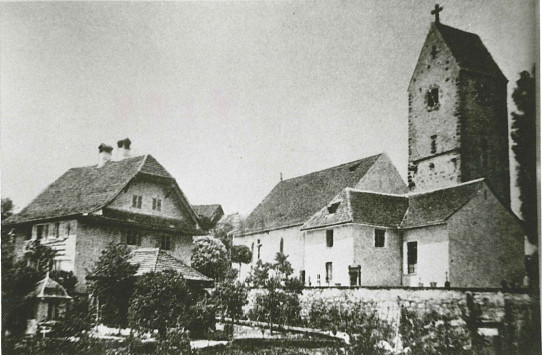
\includegraphics[width=0.45\textwidth]{./Dorf-Bilder/Alte-Kirche-mit-Pfarrhaus.jpg}%

    }\hfil \subfloat[Gasthof zum roten Löwen]{%
        \includegraphics[width=0.45\textwidth]{./Dorf-Bilder/Löwen-vor-1900.jpg}%

    }\\
    \subfloat[Vierwaldstätterhof 1895]{%
        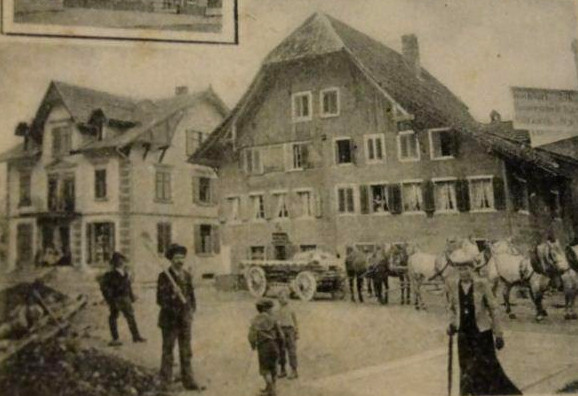
\includegraphics[width=0.45\textwidth]{./Dorf-Bilder/Dorfplatz-1895.jpg}%
    }\hfil \subfloat[Dorfplatz]{%
        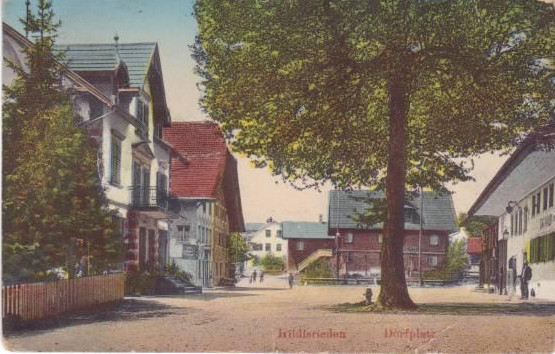
\includegraphics[width=0.45\textwidth]{./Dorf-Bilder/Dorfplatz.jpg}%
    }
\end{figure}
